\section{Wechselkurse}
\subsection{Nominaler Wechselkurs}
Erhöht sich die inländische Geldmenge im Vergleich zur ausländischen, dann steigt der nominale Wechselkurs. Dies ist eine Abwertung der inländischen Währung. Umgekehrt ist eine Erhöhung der ausländischen Geldmenge eine Aufwertung der inländischen Währung. 
\begin{equation*}
 e\quad\text{(nominaler Wechselkurs)} = \frac{\text{inländische  Währung}}{\text{ausländische Währung}}
\end{equation*}
\subsection{Realer Wechselkurs}
Bei den realen Wechselkursen werden die unterschiedlichen Preisniveaus im Inland und Ausland berücksichtigt.
\begin{equation*}
	r\quad \text{(realer Wechselkurs)} = \frac{e \cdot p^{*}\quad \text{(Preis Güterkorb  im Ausland in  ausländischer  Währung)}}{p\quad \text{(Preis\ Güterkorb im Inland in inländischer Währung})}
\end{equation*}
\begin{itemize}
	\item Erhöhung inländische Geldmenge
	\subitem Nominaler Wechselkurs steigt sofort
	\subitem Langfristig ändert realer Wechselkurs nicht, da sich Preisniveau anpasst
\end{itemize}

Wenn r > 1 ist der Güterkorb im Ausland teurer.
\clearpage
\pagebreak
\subsection{Fixe Wechselkurssysteme}
\begin{itemize}
	\item Berechnbarkeit des Wechselkurs
	\item Anbindung der eigenen Geldpolitik an stabilere Geldpolitik
	\item Vereinfacht Handelsbeziehungen
	\item Keine Möglichkeit zur Konjunktursteuerung
	\item Bei der EWS (Europäische Währungssystem, Leitwährung D-Mark) gibt es in den Ländern unterschiedliche Inflationsraten und Konjunkturzyklen, daher sind fixe Wechselkurse ein Problem
\end{itemize}
\subsection{Währungsunion}
\begin{itemize}
	\item In der Währungsunion sind die nominalen Wechselkurse fixiert durch eine Zentralbank
	\item In einem fixen Wechselkurssystem sind die Kurse nicht für alle Zeiten fixiert. Jedes Land kann aus dem System aussteigen
	\item Keine Wechselkursrisiko
	\item Erhöhung der Preistransparenz, da Güterkorbpreise direkt verglichen werden können.
	\item Falls die Länder trotzdem konjunkturell unterschiedlich sind sollte dies durch flexible Löhne, Preise, mobile Arbeitskräfte und ausgleichende Fiskalströme aufgefangen werden. 
	\item Dies funktioniert aber in der EWU (Europäischer Währungsunion, Vertrag von Maastricht) nicht.
	\item Dadurch bauten sich makroökonomische Ungleichgewichte auf. Alle Mitgliedsstaaten konnten sich zu den gleichen Zinsen verschulden. Für die PIGS-Staaten war dies eine billige Verschuldung (Zinsen tief). Dies ist der Grund für die Eurokrise.
\end{itemize}
\begin{figure*}[h]
\centering
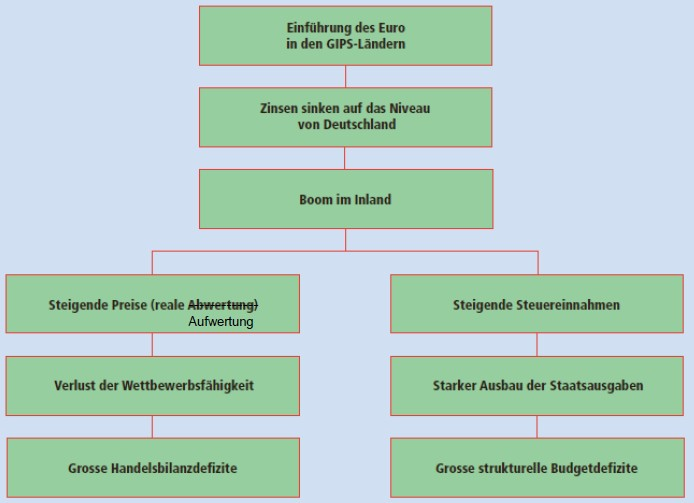
\includegraphics[width=0.8\linewidth]{images/eurokrise.jpg}
\end{figure*}
\begin{minipage}{0.5\linewidth}
Verlust der Wettbewerbsfähigkeit:
\[ r\downarrow = \frac{e \cdot p^*}{p\uparrow} \]
\end{minipage}
\begin{minipage}{0.5\linewidth}
    Strukturelle Budgetdefiziete nach Einbruch der Steuereinnahme
\end{minipage}
\clearpage
\pagebreak